\documentclass[a4paper]{article} 
\usepackage[dutch]{babel}
\usepackage{graphicx}
\usepackage{color}
\usepackage[final]{pdfpages}
\usepackage{hyperref}

\usepackage[margin=2.9cm]{geometry} %ik denk dat de we wel een redelijk aantal paginas gaan hebben wanneer het verslag klaar is, de standaardmarges van latex zijn echt wel groot
%\usepackage[utf8x]{inputenc} uitgeschakelt aangezien ik dit package niet heb, gebruik escape codes of hercompile de pdf zelf om speciale tekens te gebruiken


\title{SWOP - Hospitaal Iteratie 3}
\author{Groep12\\ \\Jeroen Van Gool\\Ruben Lapauw\\Tom De Bie\\Jeroen De Coninck}
\date{}
\pdfinfo{
	/Title (SWOP - Hospitaal Iteratie 3)
	/Author	(Groep\ 12)
}

\begin{document}
\maketitle
\newpage
\tableofcontents
\newpage

\section{Inleiding}
\subsection{Overzicht van het verslag}

\subsection{Veronderstellingen \label{sec:assumptions}}
\begin{itemize}
\item ''Een pati\"ent kan aan niet meer dan 10 X-ray scans per jaar onderworpen worden.'' 
Hierbij hebben we natuurlijk aangenomen dat het over de tijdspanne van een jaar gaat, 
en niet over een kalenderjaar.
Dit is natuurlijk gemakkelijk aanpasbaar.
\item Personeelsleden alsook pati\"enten hebben een unieke naam. 
Je kan echter wel een pati\"ent hebben met dezelfde naam als iemand van het personeel, 
dit leek ons logisch aangezien een personeelslid ook opgenomen kan worden in het ziekenhuis als hij of zij zelf ziek is.
\item De FIFO-queue wordt nu gebruikt zoals gevraagd. Dit was geen probleem met de implementatie.
\item Bij het doorspoelen van de tijd wordt als het eten op is geen eten meer gegeven aan de pati\"enten.
\item De Stock van alle items is voldoende groot dat er niet meer items gevraagd worden dan dat het minste aantal items die in een Stock kan ziten zonder dat er bijbesteld moet worden. Met andere woorden, deze is voldoende groot dat  2 dagen na de laatste afspraak altijd voldoende items zullen zijn.
\end{itemize}
\section{Het systeem}
\subsection{Overzicht} %Informatie in het systeem.???
Het hospitaal heeft verschillende subsystemen: 
De wereld die als oer-Object dient. 
Deze houdt de tijd, personen, machines en voorraad bij. 
De personen splitsen zich op in patienten en personeel. 
Het personeel kan verschillende operaties uitvoeren op het systeem. 
Terwijl er op patienten operaties worden uitgevoerd: 
Voeg diagnoses, medische testen en behandelingen toe. 
Medische testen en behandelingen hebben allebei een afspraak die als alle andere precondities voldaan zijn gemaakt worden. 
Verder is er nog voorraad. Deze voorziet maaltijden voor de patienten en andere items voor de behandelingen. 
De bestellingen gebeuren hiervan automatisch. Bestellingen worden niet automatisch verwerkt.


\subsection{Gebruikers \label{sec:users}}
\subsubsection{Usecases: Login, Logout}
De enige verandering is de keuze van een Campus bij het inloggen. 
Dit gebeurt aan de hand van CampusInfo's die worden gevraagd aan de World. 
In de CampusInfo zit enkel de naam van de Campus en daardoor kan de Campus niet onnodig gewijzigd worden door de Login. 
Vervolgens wordt in de login methode van WorldController de Campus weer opgevraagd aan de World via zijn CampusInfo. 
Ten slotte wordt er een CampusController aangemaakt die de juiste Campus bijhoudt, 
deze wordt gebruikt door LoginControllers, zoals bv. de DoctorController of de NurseController.
Bij logout is er niets veranderd.
	
\subsubsection{Bespreking GRASP, uitbreidbaarheid en nadelen}
Dit was een eenvoudige aanpassing. Dezelfde opmerkingen als bij de vorige iteratie zijn van toepassing.

\subsection{Input en output}
\subsubsection{Beschrijving}
Input en output is is strikt gereguleerd. Alle output moet ofwel immutable zijn, zoals Strings en andere, ofwel read-only, zoals CampusInfo en LoginInfo, ... 
Voor Input moet men ook oppassen: deze moet ook immutable zijn, ofwel moet men een perfecte kopie maken van alle Objecten die ingegeven worden. Maar alleen met primitieven en Strings werken is niet uitbreidbaar en onhandig werken.
Men kan bijvoorbeeld niet garanderen dat alle behandelingen hetzelfde aantal parameters hebben van hetzelfde type. 
De oplossing is om de parameters te abstraheren naar een Object Argument. 
Om de kennis van in het systeem dan ook nog af te schermen van de UI is er een vraag bij gegeven. Hierdoor moet de UI niet de vragen stellen aan de gebruiker en kunnen gemakkelijk nieuwe behandelingen met andere parameters toegevoegd worden. Een andere gevolg is dat men direct kan controleren of de invoer mogelijks correct is.

\subsubsection{Publieke Werking}
De interface PublicArgument<E> is de basis van de invoer. Deze heeft een vraag die aan de gebruiker moet gevraagd worden. En deze kan beantwoord worden door de setAnswer methode met een String. Deze wordt direct geconverteerd naar het type E. Deze Argumenten zitten in een ArgumentList, samen met objecten van de superklasse Argument<E>. Deze objecten zijn voor het interne systeem om in te vullen, op het moment dat de UI de controle teruggeeft aan het systeem.  

\subsubsection{Interne Werking}
Een generische factory verwacht als invoer om een nieuw object te maken een lijst van Arguments. Men kan een nieuwe lege lijst Argumenten opvragen aan deze factory met de methode getEmptyArgumentList. Als deze ingevuld is door de UI en door de andere code wordt de make-methode aangeroepen met deze lijst. Deze doet dan de specifieke inputvalidation. Met de validate-methode kan gecontroleerd worden of een lijst correct is voor een bepaalde factory zonder een object te maken.

\subsubsection{Bespreking GRASP en uitbreidbaarheid}
Deze opbouw laat toe om een grote diversiteit aan invoer uit te lezen op een veilige EN generische manier. Het laat toe om de input statisch te valideren tijdens de invoer en zo duidelijker fouten terug te geven. Wat de cohesie ten goede komt. Het laat ook toe om informatie van het systeem te lezen zonder dat de UI deze zelf moet zoeken. Hierdoor is de koppeling tussen de UI en het systeem lager en duidelijk herkenbaar. 

Men kan eenvoudigweg nieuwe argumenten ontwerpen en gebruiken zonder dat er iets moet veranderen aan de UI. Om informatie van andere objecten mee te geven kan men gebruik maken van het visitor-pattern en een filter.

\subsection{Magazijn}
\subsubsection{Beschrijving}
Hier volgt een overzicht van de belangrijkste klasse en een korte beschrijving van hun taken in ons ontwerp van het magazijn systeem:
\begin{itemize}
\item LIFO-queue: Dit is een FIFO-queue geworden zoals voorzien.
\item FIFO-queue: Een wrapper rond Queue<E> en geabstraheerd als ItemQueue.
\item ItemReservator: Deze klasse is verwijderd. En is vervangen door de ItemReservationCommand. Deze heeft een andere naam en andere verantwoordelijkheden.
\item ReserveItemObserver: Deze klasse is verwijderd, een afspraak wordt direct gepland op het moment dat alle items beschikbaar zijn.
\item ItemReservationCommand: Deze klasse reserveert alle nodige items in een stock. Op het moment van de afspraak komen de Items in deze klasse beschikbaar.
\item ItemInfo: Dit object is een veilig object om buiten het systeem te gebruiken. 
\item ItemConstraint: Deze constraint wordt bij het maken van een afspraak in rekening gebracht om een goed moment van afspraak te vinden.
\end{itemize}

\subsubsection{Interne Werking}
In tegenstelling tot de vorige iteratie wordt een afspraak nu wel direct gepland. Een geschiedenis van alle afspraken wordt voor ieder item bijgehouden en bij het plannen van de afspraak wordt een moment gezocht waar  er geen tekort aan items is, noch waar er ooit in de toekomst problemen zullen komen. Het gebruik van een Item kan zich ver in de toekomst propageren en zo binnen een aantal maanden een probleem veroorzaken. 
\subsubsection{Bespreking GRASP}
De twee subsystemen, het Warehouse en de Scheduler, zijn enkel met een Constraint verbonden. Dit garandeerd een minimale koppeling. De constraint zelf bevat ook weinig logica en wordt door een afgescheiden algoritme afgehandeld die apart getest kan worden.
\subsubsection{Nadelen}
Bij het plannen wordt geen rekening gehouden met het eventuele vervallen van de items aangezien we dit niet kunnen voorspellen. Het gebruik van een FIFO-queue en een ``druk'' hospitaal zorgen ervoor dat deze kans klein is. 

\subsection{Medische testen en behandelingen \label{sec:medicaltest} \label{sec:treatment}}
\subsubsection{Verloop usecases: OrderMedicalTest en EnterTreatment}
Bij deze usecases is er een grote aanpassing. Namelijk het gebruik van preemptive-scheduling. Het eerste zal apart in de sectie Scheduling\ref{sec:scheduling} worden uitgelegd. De prioriteit van deze Appointment wordt gevraagd via een PriorityArgument.
\subsubsection{Bespreking GRASP en uitbreidbaarheid}
Aan de usecase zelf is niets veranderd. De UI heeft geen enkele verandering in gedrag.

\subsection{Tijdsplanning \label{sec:scheduling}}
\subsubsection{Beschrijving}
Afspraken worden gemaakt voor een Appointable, dit wordt gedaan door AppointmentFactory. Deze zoekt een moment waarop alle constraints voldaan zijn. Ook is de eerste constraint een GetCampusConstraint voor ieder type van afspraak: deze bepaalt de campus waarop deze zich zal voordoen.

Voor een afspraak tussen een docter en een patient moeten bijvoorbeeld aan volgende Constraints voldaan zijn: 
DoctorBackToBackConstraint (DoctorPatientAppointment), Preference (van Doctor), PriorityConstraint (DoctorPatientAppointment),  en WorkingHoursConstraint (Doctor). 
Elk van deze constraints maken deel uit van alle voorwaarden die opgelegd zijn aan de afspraken. 
De PriorityConstraint zorgt dat er geen twee appointments op hetzelfde moment vallen en als er op een afspraak op dat moment staat bij een persoon dat die een lagere prioriteit heeft en dus zal verzet worden. De DoctorBackToBackConstraint zorgt ervoor dat de afspraak ofwel op het uur valt ofwel dat de afspraak direct na de vorige valt.

\subsubsection{Bespreking GRASP en uitbreidbaarheid}
De koppeling tussen de twee belangrijkste systemen is hier laag: De scheduler weet niet eens dat er iets in de warehouse gedaan wordt. En behalve dat het opvragen van alle benodigde informatie is alles afgeschermd.  De scheduler weet enkel dat hij constraints opvraagt van een Schedulable, en van een Appointable. 

Het algoritme is ook afgeschermd in een eigen deel binnen dit systeem. Dit laat toe om snellere algoritmes te gebruiken, zoals constraintprocessing met backjumping, ...

\subsection{Preference}
Deze usecase is eenvoudig. Een ListArgument van alle beschrijvingen van preferences worden opgevraagd en dan deze set dan de preference van de doctor. De PreferenceConstraint vraagt deze op en controleert alle mogelijke momenten met deze preference. Om een nieuwe preference te maken moet men een klasse maken die de interface Preference uitbreidt.

\section{Onveranderde Usecases}
Aan de volgende Usecases is er niets veranderd:
\begin{itemize}
 \item Undo \& Redo: Deze interfaces is volledig hetzelfde.
 \item Consult Patientfile
 \item Close Patientfile
 \item Discharge Patient
 \item Register Patient
 \item Enter MedicalTestResult
 \item Fill Stock
 \item List Orders
 \item Enter Diagnosis
 \item AddEquipment: Voor deze usecase is er niets veranderd, de factories hebben gewoon een CampusInfoArgument gekregen zodat deze automatisch wordt ingevuld in de UI.
 \item AddStaffMembers: zie AddEquipment
\end{itemize}

\subsection{Enter TreatmentResult}
Door het gebruik van een geschiedenis in het Warehouse kunnen resultaten pas ingevuld worden wanneer de items er uit verwijderd zijn. En dit mag enkel op het juiste moment, anders kan zal de planning niet meer juist werken. Het is dus logisch dat resultaten pas uitgevoerd kunnen worden als het na de start van deze afspraak is. Anderzijds moet men tijdens het vooruitspoelen van de tijd direct de resultaten opschrijven van alle afspraken die geweest zijn. Dit zou betekenen dat men als zuster enkel de tijd heeft om deze in te vullen voor het einde van de afspraak. We hebben gekozen om AdvanceTime op een logischere manier te laten werken en toch niet te veel van de opgave af te wijken.

\subsection{Advance Time}
Door de veranderingen die gebeurd zijn aan het Warehouse was het niet logisch om results in te vullen als meteen wanneer deze verlopen. De aanpassing is gemaakt dat deze moeten ingevuld worden voor het einde van de dag en anders door de HospitalAdministrator. Verder gebeurt AdvanceTime op dezelfde manier als in iteratie 2. 

\section{Conclusie}
De uitbreidbaarheid van ons systeem in hetzelfde gebleven. De gevonden pijnpunten van de vorige iteratie zijn verbeterd. De verscheidenheid aan constraints bij het schedulen is groter geworden zoals verwacht en zonder grote aanpassingen. 


\section{Appendices}
%\subsection{Mogelijke uitbreidingen} wordt eigelijk al besproken in de conclusie
\subsection{De user interface \label{sec:ui}}
De UI is niet veranderd. Er is een methode voor de nieuwe usecase Selet Preference bijgekomen.

\subsection{Testverslag}
\subsubsection{Teststrategie}
Het testen is voortgezet geweest zoals in het vorige semester. Er zijn een aantal scenarios opgesteld die de volledige API testen, in andere tests wordt een deel van de API getest. Het schedulen van afspraken is uitvoerig getest geweest. Alle constraints worden getest op uitzonderingsgevallen. Ook de AppointmentConstraintSolver werd getest.

Dit is zoals voorzien in ons testverslag van vorig semester.

\subsubsection{Eclemma-verslag} %het verslag zelf moet hier nog bijgevoegd worden
Eclemma rapporteert in tegenstelling tot iteratie 2 een redelijke converage van 70\%. Dit komt omdat de code van de UI afgescheiden is geweest naar een apart project. Ook zijn ongebruikte klassen verwijderd of in gebruik genomen, met de nodige testen.

op het eerste zicht een slechte testsuite. Wanneer we echter in detail kijken naar het verslag, zien we dat de slechtst gecoverde klassen de UI- en exception klassen zijn. De UI-klassen zijn niet opgenomen in de tests, en de exceptions voorzien vaak alternatieve constructors (met/zonder message) die niet altijd gebruikt worden. Daarbovenop is er in de gewone klassen ook vaak error-handling code voor exceptions die technisch gezien niet voor zouden kunnen komen, of door overerving vereiste methoden die niet gebruikt worden, logischerwijs wordt deze code ook niet covered door de testen waardoor het totale coverage-percentage daalt.

Echter de beste aanduiding van de kwaliteit van onze testsuite is het feit dat doorheen het implementeren van de software we gebruik hebben kunnen maken van onze tests om fouten in het systeem te kunnen opsporen. Deze ervaring van nut uit de tests gehaald te kunnen hebben zonder onzekerheid of het systeem nu wel \'echt werkt is waarschijnlijk ook de beste indicator voor testsuite-kwaliteit.

\begin{figure}[h]
\centering
\caption{Eclemma code coverage verslag voor de testsuite}
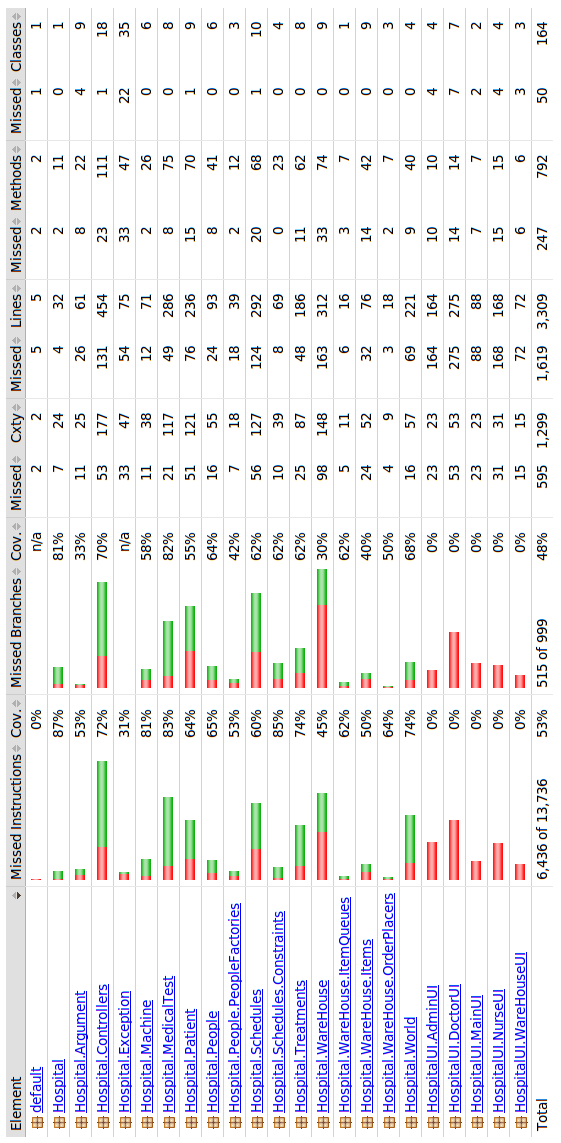
\includegraphics[height=\textheight]{Pictures/Eclemma}
\label{fig:eclemma}
\end{figure}
\subsection{Werkverdeling} %dit moet gewoon een tabel worden zeker? (met de uren en onderwerpen van het werk van iedereen)
\begin{center}
\begin{tabular}{| r || c | l |}
\hline
De Bie Tom & nog door te geven & <voeg lijst in> \\
\hline
De Coninck Jeroen & nog door te geven & Refactoring \\
\hline
Lapauw Ruben & \~ 56 uur & Scheduling, AddEquipment \& AddStaffMembers \\
	     &		 & Warehouse, Verslag \\
\hline
Van Gool Jeroen & nog door te geven & <voeg lijst in> \\ %Probeer nog eens ... %& 60 & Diagnoses \& MedicalTest \\
~ & ~ & Verslag \\
\hline
\end{tabular}
\end{center}
\newpage
\subsection{Volledig klassendiagram \label{sec:classdiagram}}
druk dit apart af gespreid over 2 paginas en voeg in in plaats van dit blad
\newpage
\end{document}
